%%%%%%%%%%%%%%%%%%%%%%%%%%%%%%%%%%%%%%%%%%%%%%%%%%%%%%%%%%%%%%%%%%%%%%%%%%
% Signals of u2,p u2,m for raising load
%%%%%%%%%%%%%%%%%%%%%%%%%%%%%%%%%%%%%%%%%%%%%%%%%%%%%%%%%%%%%%%%%%%%%%%%%%
\begin{solutionfigure}[htb]

 %   \documentclass{standalone}
 %   \usepackage{pgfplots}
 %   \pgfplotsset{compat=1.18} % Kompatibilität für neuere Versionen
        \centering
        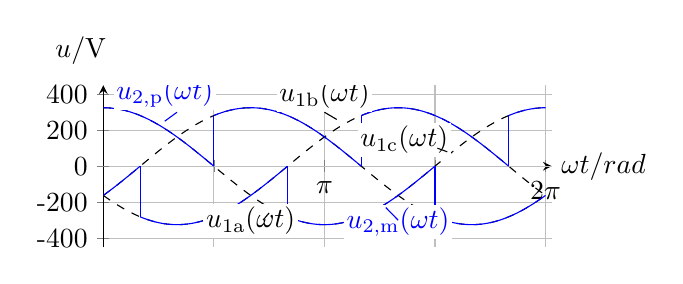
\begin{tikzpicture}
            \begin{axis}[
                % x/y range adjustment
                xmin=0, xmax=365,
                ymin=-450, ymax=450,
                samples=500,
                axis y line=center,
                axis x line=middle,
                extra y ticks=0,
                % Label text
                xlabel={$\omega t / \text{rad}$},,
                ylabel={$u/\mathrm{V}$},
                % Label adjustment
                x label style={at={(axis description cs:1,0.5)},anchor=west},
                y label style={at={(axis description cs:-.05,.97)},anchor=south,yshift=0.2cm},
                width=0.6\textwidth,
                height=0.3\textwidth,
                % x-Ticks
                xtick={0,90,180,270,360},
                xticklabels={,,$\pi$,,$2\pi$},
                xticklabel style = {anchor=north},
                % y-Ticks
                ytick={400,200,0,-200,-400},
                yticklabels={400,200,0,-200,-400},
                yticklabel style = {anchor=east},
                % Grid layout
                grid,
                %grid style={line width=.1pt, draw=gray!10},
                %major grid style={line width=.2pt,draw=gray!90},
            ]
            % Voltage u1a(wt), u1b(wt) u1c(wt)
            \addplot[black, domain= 0:360,dashed] {325*cos(x)};                
            \addplot[black, domain= 0:360,dashed] {325*cos(x+120)};                
            \addplot[black, domain= 0:360,dashed] {325*cos(x+240)}; 
            % Voltage u2p(wt)
            \addplot[blue, domain= 0:90] {325*cos(x)};                
            \addplot[blue, domain= 90:210] {325*cos(x+240)};                
            \addplot[blue, domain= 210:330] {325*cos(x+120)};
            \addplot[blue, domain= 330:360] {325*cos(x)};                
            \addplot[color=blue,solid] coordinates{
                (90,0)
                (90, 281.4)
            };     
            \addplot[color=blue,solid] coordinates{
                (210,0)
                (210, 281.4)
            };     
            \addplot[color=blue,solid] coordinates{
                (330,0)
                (330, 281.4)
            };     
         
            % Voltage u2m(wt)
            \addplot[blue, domain= 0:30] {325*cos(x+240)};                
            \addplot[blue, domain= 30:150] {325*cos(x+120)};                
            \addplot[blue, domain= 150:270] {325*cos(x)};                
            \addplot[blue, domain= 270:360] {325*cos(x+240)};
            \addplot[color=blue,solid] coordinates{
                (30,0)
                (30, -281.4)
            };     
            \addplot[color=blue,solid] coordinates{
                (150,0)
                (150, -281.4)
            };     
            \addplot[color=blue,solid] coordinates{
                (270,0)
                (270, -281.4)
            };     
        
            % Label of u1c
            \node[black, fill=white, inner sep = 1pt, anchor = south] at (axis cs:245,50) {$u_{\mathrm{1c}}(\omega t)$};
            % Line to u1a
            \draw[thin, black] (272,100) -- (280,80); 
            % Label of u1a
            \node[black, fill=white, inner sep = 1pt, anchor = south] at (axis cs:120,-400) {$u_{\mathrm{1a}}(\omega t)$};
            % Line to u1a
            \draw[thin, black] (130,-300) -- (135,-260);            
            % Label of u1b
            \node[black, fill=white, inner sep = 1pt, anchor = south] at (axis cs:180,300) {$u_{\mathrm{1b}}(\omega t)$};
            % Line to u1b
            \draw[thin, black] (180,300) -- (190,260);
            % Label of u2,p
            \node[blue, fill=white, inner sep = 1pt, anchor = south] at (axis cs:50,310) {$u_{\mathrm{2,p}}(\omega t)$};
            % Line to u2,p
            \draw[thin, blue] (60,300) -- (50,250);
            % Label of u2,m
            \node[blue, fill=white, inner sep = 1pt, anchor = south] at (axis cs:240,-410) {$u_{\mathrm{2,m}}(\omega t)$};
            % Line to u2,m
            \draw[thin, blue] (240,-300) -- (230,-230);
        \end{axis}     
        \end{tikzpicture}
        \caption{Output voltage $u_\mathrm{2,p}(t)$ and $u_\mathrm{2,m}(t)$ for raising load.}
        \label{sfig:ex06_Voltage_u2pmn_Raise}
\end{solutionfigure}